\documentclass{beamer}
% \usetheme{tau}
\usetheme{Madrid}

%------------------------------------------------------------
%This block of code defines the information to appear in the
%Title page
\title[Deep Learning in Medical Imaging Seminar]{Infinite Brain Tumor Images: Can GAN-based Data Augmentation Improve Tumor Detection on MR Images?}
\subtitle{\footnotesize Changhee Han, Leonardo Rundo, Ryosuke Araki, Yujiro Furukawa, Giancarlo Mauri, Hideki Nakayama, Hideaki Hayashi}

\author[Mahler, Zaltzman]{Tom~Mahler\inst{1} \and Amir~Zaltzman\inst{2}}
% \institute{Deep Learning in Medical Imaging}

\institute[BGU, TAU] % (optional)
{
  \inst{1}%
  Faculty of Software and Information Systems Engineering\\
  Ben-Gurion University of the Negev
  \and
  \inst{2}%
  Faculty of Electrical Engineering\\
  Tel Aviv University
}

\date[May 2019] % (optional)
{Deep Learning in Medical Imaging, May 2019}

\logo{
\includegraphics{taufront.png}}

%End of title page configuration block
%------------------------------------------------------------

%------------------------------------------------------------
%The next block of commands puts the table of contents at the 
%beginning of each section and highlights the current section:

\AtBeginSection[]
{
  \begin{frame}
    \frametitle{Table of Contents}
    \tableofcontents[currentsection]
  \end{frame}
}
%------------------------------------------------------------



\begin{document}

%The next statement creates the title page.
\frame{\titlepage}

% \begin{frame}
% \titlepage
% \end{frame}

%---------------------------------------------------------
%This block of code is for the table of contents after
%the title page
\begin{frame}
\frametitle{Table of Contents}
\tableofcontents
\end{frame}
%---------------------------------------------------------


% Prepare a 12 minute presentation  (10-15 slides)
% The seminar should cover the following items:  
% TOPIC of Research + Full Reference list: Article Title, Author list, Journal name, Year 





\section{Motivation \& Problem Statement}
% What exactly are the authors working on? What is the scope of the project?
%---------------------------------------------------------
%Motivation \& Problem Statement
\begin{frame}
\frametitle{Motivation \& Problem Statement}
\begin{figure}
   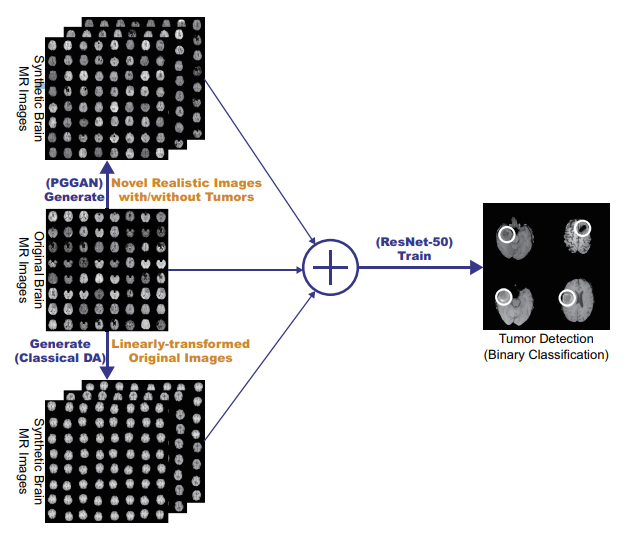
\includegraphics[width=5cm]{img/PGGAN-based_DA}
\end{figure}

The authors are working on ...\\
The scope of the project is ...
\end{frame}
%---------------------------------------------------------


\section{Previous Work}
% What is the state of the art, and how the current article relates to the state of the art (see if you can get some info from the additional articles you extracted).
%---------------------------------------------------------
%Previous Work
\begin{frame}
\frametitle{Previous Work}
The state of the art is ...\\
The current article relates to the state of the art ...
\end{frame}
%---------------------------------------------------------


\section{Describe the Methods}
% (short outline) What is used and why? What were the other choices possible? Are there items that can be critiqued in the methods?
%---------------------------------------------------------
%Describe the Methods
\begin{frame}
\frametitle{Describe the Methods}
... is used because ...

The other choices possible were...

The items that can be critiqued in the methods are ...

\end{frame}
%---------------------------------------------------------

\section{Describe the Experiments}
% (short outline) What is the goal of the experiments? What is the experimental design? Is it good/bad?
%---------------------------------------------------------
%Describe the Experiments
\begin{frame}
\frametitle{Describe the Experiments}
The goal of the experiments is ...

The experimental design is ... and it is good/bad because ...

\end{frame}
%---------------------------------------------------------

\section{Results and Discussion}
% Are the results good/bad? How are they interpreted? Do you agree? 
%---------------------------------------------------------
%Results and Discussion
\begin{frame}
\frametitle{Results and Discussion}
The results good/bad ...

They are interpreted in the following way ...

We agree/disagree because ...

\end{frame}
%---------------------------------------------------------

\section{Our Suggestions}
% Suggest ways in which you suggest to improve the system you researched; suggest an improved algorithm; possible combination across different methods etc.
%---------------------------------------------------------
%Our Suggestions
\begin{frame}
\frametitle{Our Suggestions}
We suggest to improve the system we researched as follows ....

We suggest to improve the algorithm as follows ....

We suggest to possibly combine these different methods ... as follows ....

\end{frame}
%---------------------------------------------------------


\section{Beamer Examples}

%---------------------------------------------------------
%Changing visivility of the text
\begin{frame}
\frametitle{Sample frame title}
This is a text in second frame. For the sake of showing an example.

\begin{itemize}
    \item<1-> Text visible on slide 1
    \item<2-> Text visible on slide 2
    \item<3> Text visible on slides 3
    \item<4-> Text visible on slide 4
\end{itemize}
\end{frame}
%---------------------------------------------------------

%---------------------------------------------------------
%Example of the \pause command
\begin{frame}
In this slide \pause

the text will be partially visible \pause

And finally everything will be there
\end{frame}
%---------------------------------------------------------

%---------------------------------------------------------
%Highlighting text
\begin{frame}
\frametitle{Sample frame title}

In this slide, some important text will be
\alert{highlighted} because it's important.
Please, don't abuse it.

\begin{block}{Remark}
Sample text
\end{block}

\begin{alertblock}{Important theorem}
Sample text in red box
\end{alertblock}

\begin{examples}
Sample text in green box. The title of the block is ``Examples".
\end{examples}
\end{frame}
%---------------------------------------------------------


%---------------------------------------------------------
%Two columns
\begin{frame}
\frametitle{Two-column slide}

\begin{columns}

\column{0.5\textwidth}
This is a text in first column.
$$E=mc^2$$
\begin{itemize}
\item First item
\item Second item
\end{itemize}

\column{0.5\textwidth}
This text will be in the second column
and on a second tought this is a nice looking
layout in some cases.
\end{columns}
\end{frame}
%---------------------------------------------------------


\end{document}
